\documentclass[aspectratio=169]{../latex_main/tntbeamer}  % you can pass all options of the beamer class, e.g., 'handout' or 'aspectratio=43'
\usepackage{dsfont}
\usepackage{bm}
\usepackage[english]{babel}
\usepackage[T1]{fontenc}
%\usepackage[utf8]{inputenc}
\usepackage{graphicx}
\graphicspath{ {./figures/} }
\usepackage{algorithm}
\usepackage[ruled,vlined,algo2e,linesnumbered]{algorithm2e}
\usepackage{hyperref}
\usepackage{booktabs}
\usepackage{mathtools}

\usepackage{amsmath,amssymb}

\DeclareMathOperator*{\argmax}{arg\,max}
\DeclareMathOperator*{\argmin}{arg\,min}

\usepackage{amsbsy}
\newcommand{\vect}[1]{\bm{#1}}
%\newcommand{\vect}[1]{\boldsymbol{#1}}

\usepackage{pgfplots}
\pgfplotsset{compat=1.16}
\usepackage{tikz}
\usetikzlibrary{trees} 
\usetikzlibrary{shapes.geometric}
\usetikzlibrary{positioning,shapes,shadows,arrows,calc,mindmap}
\usetikzlibrary{positioning,fadings,through}
\usetikzlibrary{decorations.pathreplacing}
\usetikzlibrary{intersections}
\pgfdeclarelayer{background}
\pgfdeclarelayer{foreground}
\pgfsetlayers{background,main,foreground}
\tikzstyle{activity}=[rectangle, draw=black, rounded corners, text centered, text width=8em]
\tikzstyle{data}=[rectangle, draw=black, text centered, text width=8em]
\tikzstyle{myarrow}=[->, thick, draw=black]

% Define the layers to draw the diagram
\pgfdeclarelayer{background}
\pgfdeclarelayer{foreground}
\pgfsetlayers{background,main,foreground}

% Requires XeLaTeX or LuaLaTeX
%\usepackage{unicode-math}

\usepackage{fontspec}
%\setsansfont{Arial}
\setsansfont{RotisSansSerifStd}[ 
Path=../latex_main/fonts/,
Extension = .otf,
UprightFont = *-Regular,  % or *-Light
BoldFont = *-ExtraBold,  % or *-Bold
ItalicFont = *-Italic
]
\setmonofont{Cascadia Mono}[
Scale=0.8
]

\renewcommand{\ttdefault}{Cascadia Mono}

% scale factor adapted; mathrm font added (Benjamin Spitschan @TNT, 2021-06-01)
%\setmathfont[Scale=1.05]{Libertinus Math}
%\setmathrm[Scale=1.05]{Libertinus Math}

% other available math fonts are (not exhaustive)
% Latin Modern Math
% XITS Math
% Libertinus Math
% Asana Math
% Fira Math
% TeX Gyre Pagella Math
% TeX Gyre Bonum Math
% TeX Gyre Schola Math
% TeX Gyre Termes Math

% Literature References
\newcommand{\lit}[2]{\href{#2}{\footnotesize\color{black!60}[#1]}}

%%% Beamer Customization
%----------------------------------------------------------------------
% (Don't) Show sections in frame header. Options: 'sections', 'sections light', empty
\setbeamertemplate{headline}{empty}

% Add header logo for normal frames
\setheaderimage{
	% 
\includegraphics[height=\logoheight]{figures/TNT_darkv4.pdf}
	
\includegraphics[height=\logoheight]{../latex_main/figures/Leibniz-AI-Academy_Logo}
	% 
\includegraphics[height=\logoheight]{figures/logo_tntluh.pdf}
}

% Header logo for title page
\settitleheaderimage{
	% 
\includegraphics[height=\logoheight]{figures/TNT_darkv4.pdf}
	
\includegraphics[height=\logoheight]{../latex_main/figures/Leibniz-AI-Academy_Logo}
	% 
\includegraphics[height=\logoheight]{figures/logo_tntluh.pdf}
}

% Title page: tntdefault 
\setbeamertemplate{title page}[tntdefault]  % or luhstyle
% Add optional title image here
%\addtitlepageimagedefault{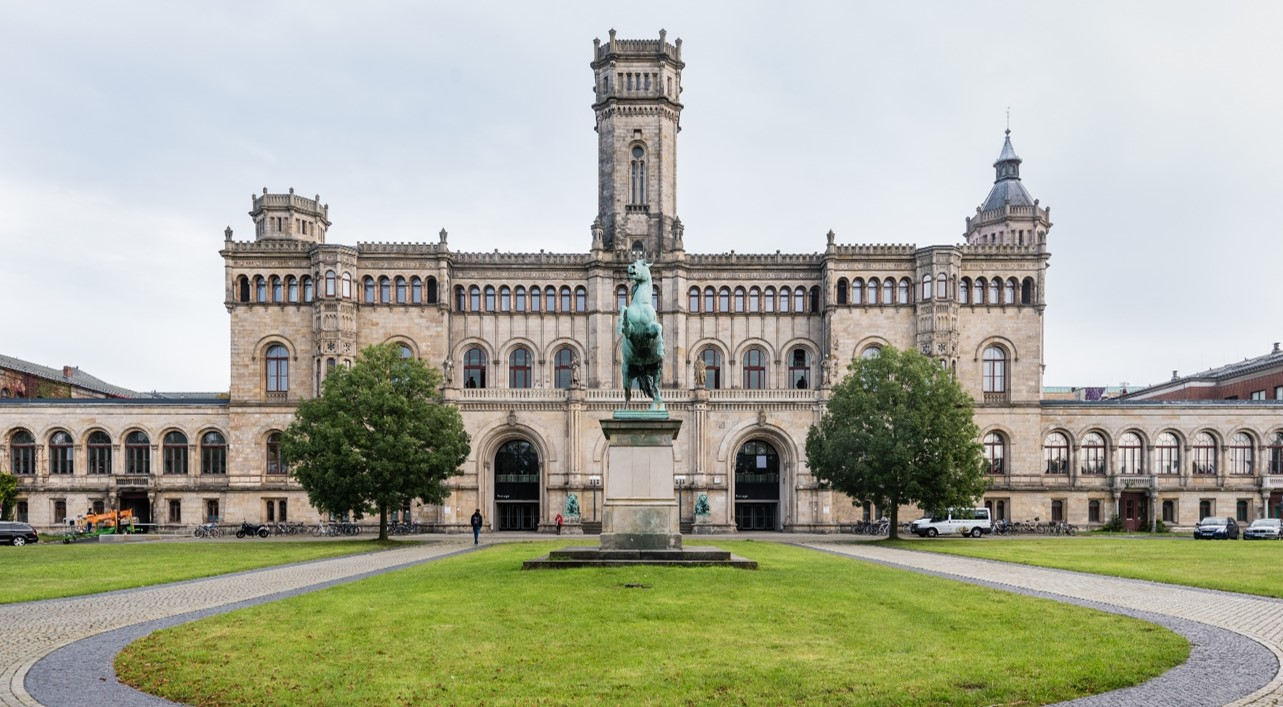
\includegraphics[width=0.65\textwidth]{figures/luh_default_presentation_title_image.jpg}}

% Title page: luhstyle
% \setbeamertemplate{title page}[luhstyle]
% % Add optional title image here
% \addtitlepageimage{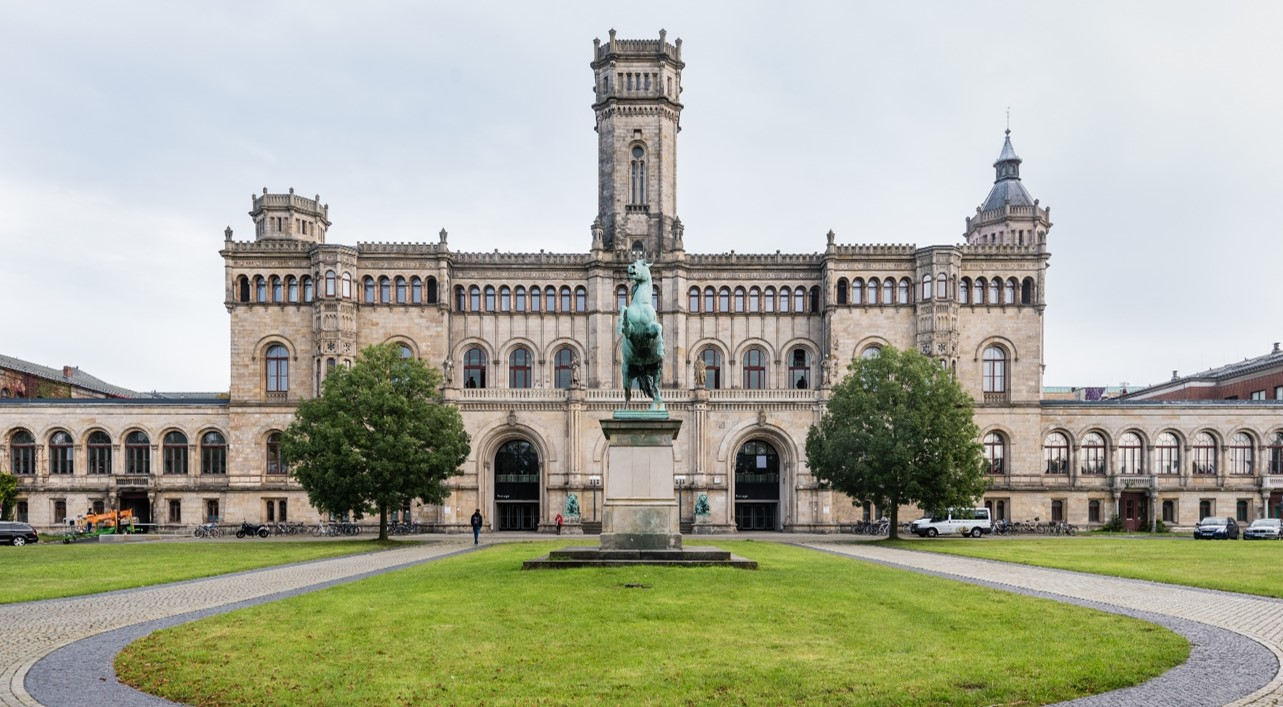
\includegraphics[width=0.75\textwidth]{figures/luh_default_presentation_title_image.jpg}}

\author[Abedjan \& Lindauer]{Ziawasch Abedjan \& \underline{Marius Lindauer}\\[1em]
	%
\includegraphics[height=\logoheight]{../latex_main/figures/luh_logo_rgb_0_80_155.pdf}\qquad
	
\includegraphics[height=\logoheight]{../latex_main/figures/DBIS_Kurzlogo.png}\qquad
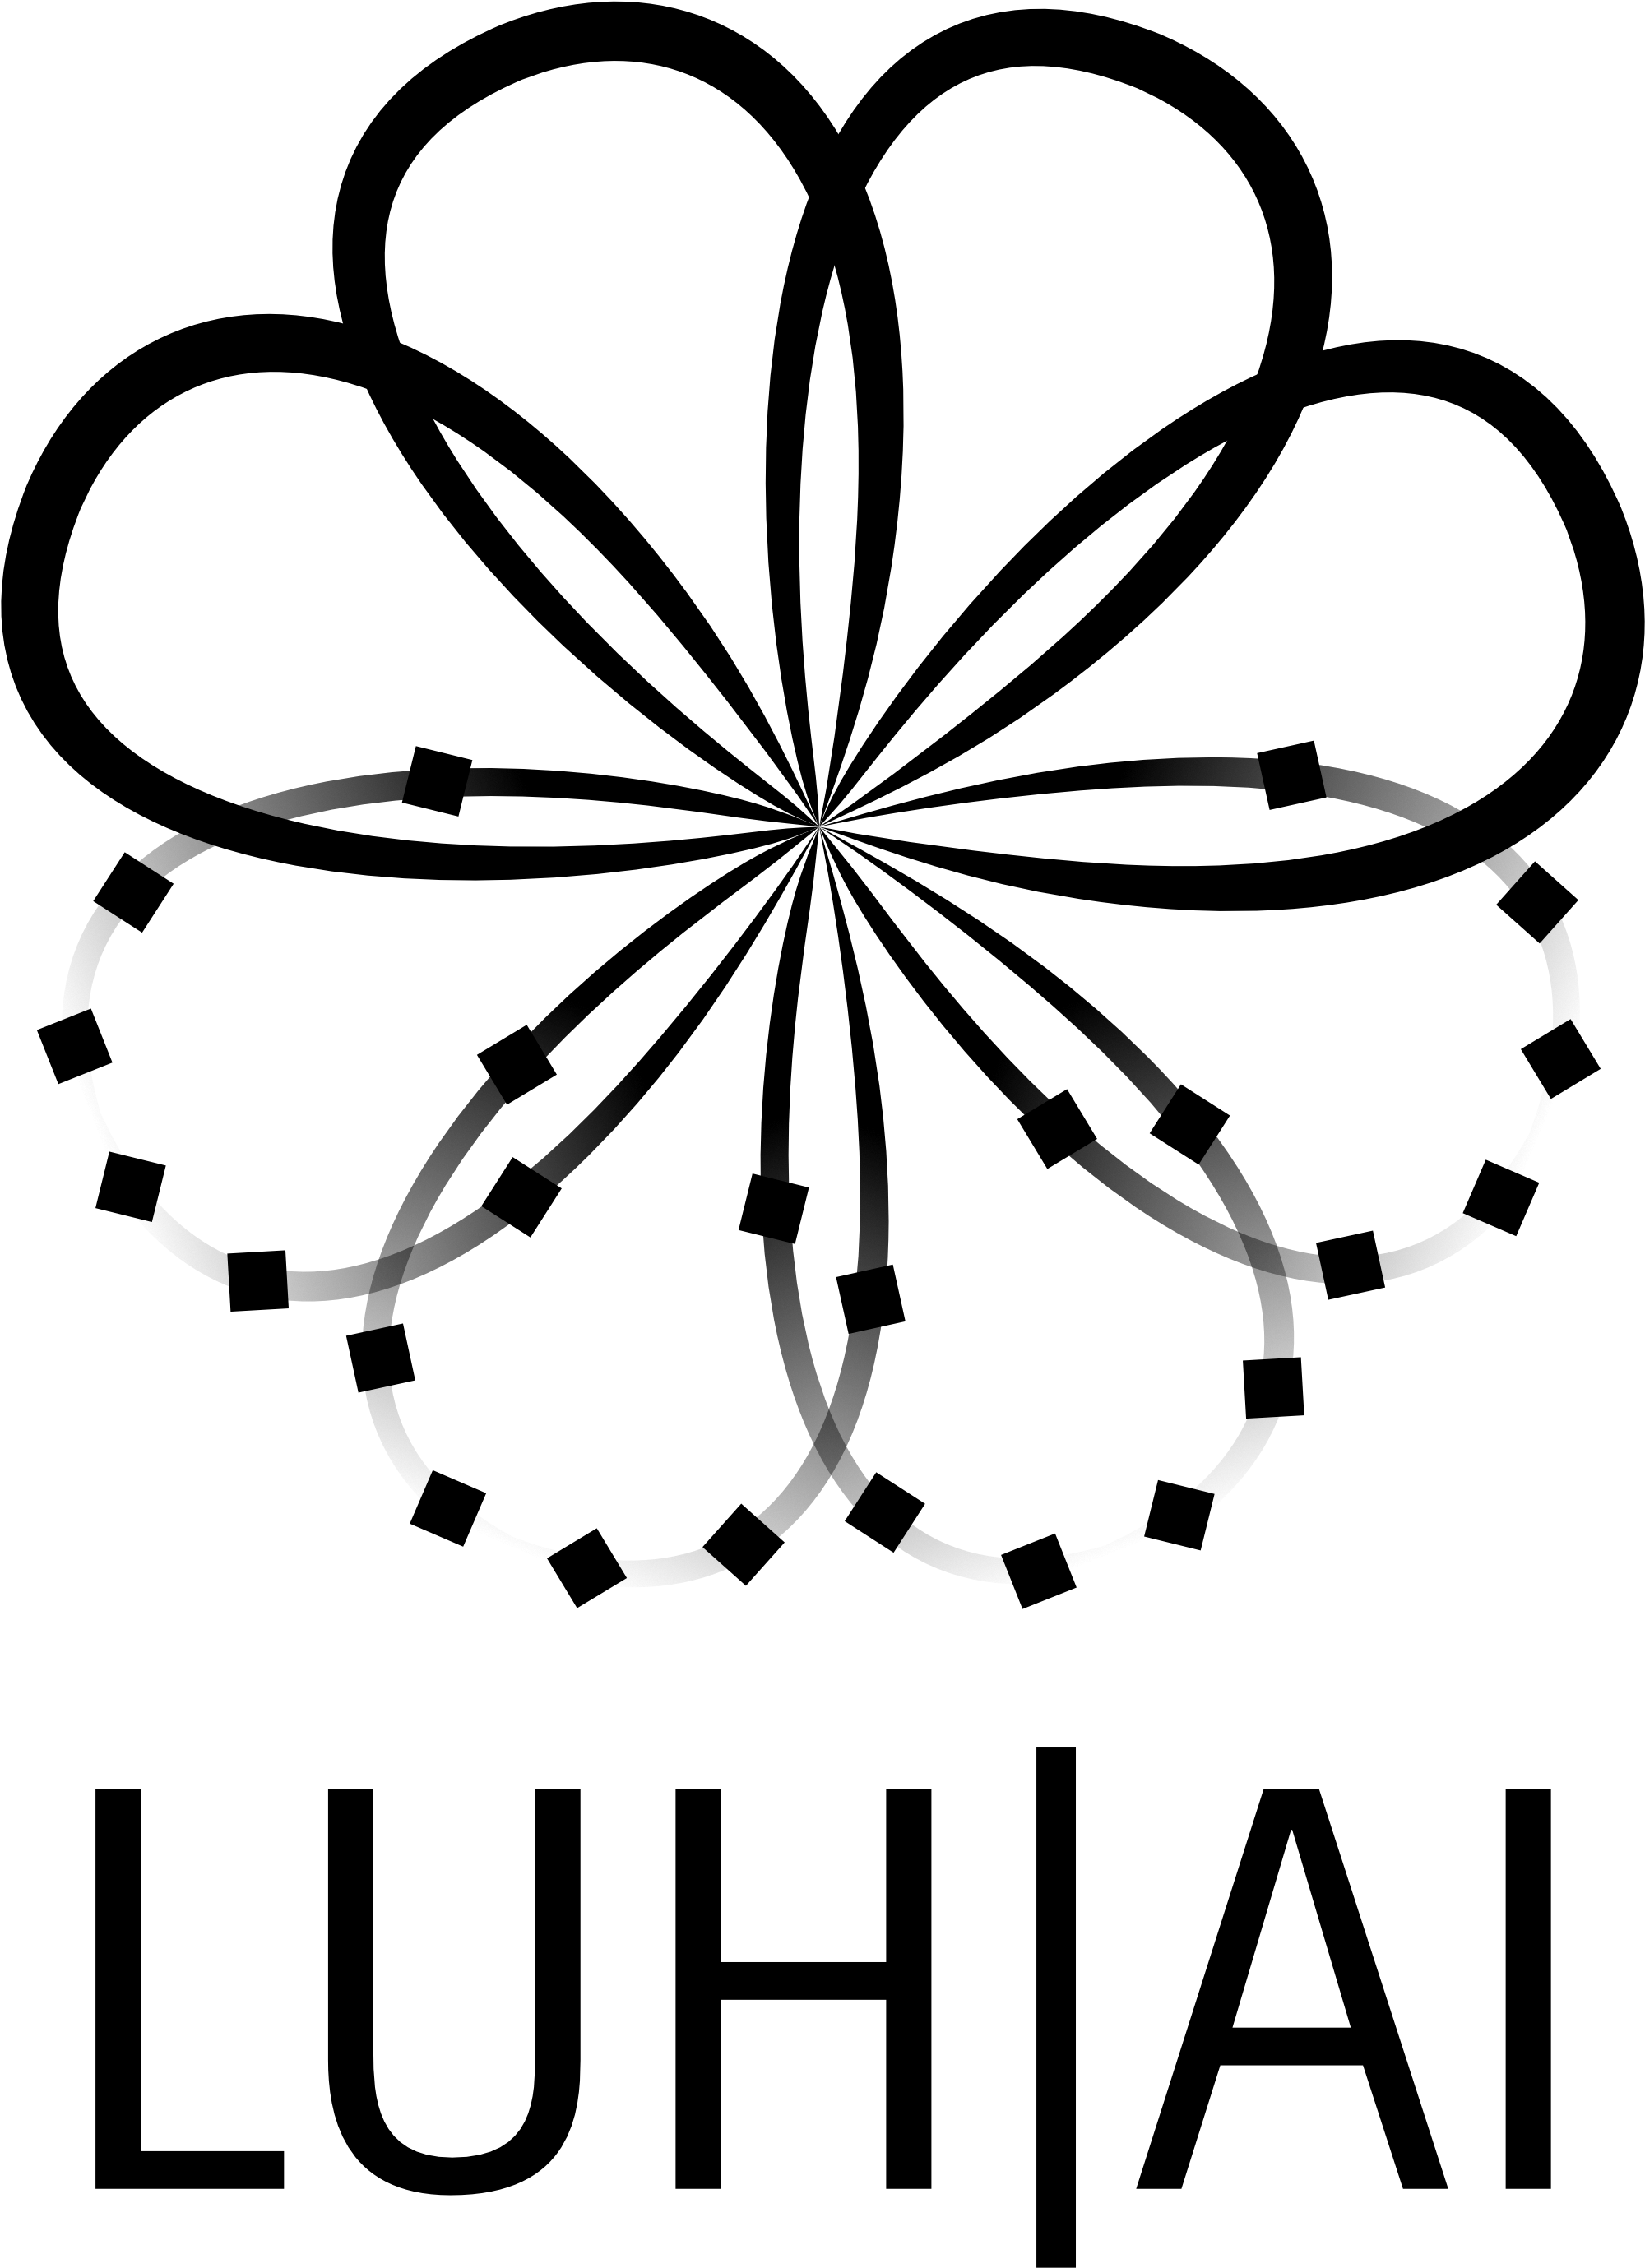
\includegraphics[height=\logoheight]{../latex_main/figures/logo_short_highres_black}\qquad

\includegraphics[height=\logoheight]{../latex_main/figures/Leibniz-AI-Academy_Logo}\qquad
%
\includegraphics[height=\logoheight]{../latex_main/figures/L3S.jpg}	
}
\date{\hspace{0.5em} {
\includegraphics[height=1.5em]{../latex_main/figures/Cc-by-nc-sa_icon.svg.png}}; extension of \href{https://ds100.org/fa21/}{[DS100]}
}


%%% Custom Packages
%----------------------------------------------------------------------
% Create dummy content
\usepackage{blindtext}

% Adds a frame with the current page layout. Just call \layout inside of a frame.
\usepackage{layout}


%%% Macros
%\renewcommand{\vec}[1]{\mathbf{#1}}
% \usepackage{bm}
%\let\vecb\bm

\title[Feature Selection]{DS: Dimension Reduction}
\subtitle{Feature Selection}

\graphicspath{ {./figure/} }
%\institute{}


\begin{document}
	
	\maketitle
	
    \begin{frame}[c]{Motivation}

    \begin{itemize}
        \item If we have too many input features, can we simply get rid of some?
        \item Use expert knowledge:
        \begin{itemize}
            \item if you, your teammates, client or other stakeholders have expert knowledge, make use of it
            \item[$\leadsto$] Remove redundant features
            \item[$\leadsto$] Remove very noisy features (or reduce noise)
            \item[$\leadsto$] Remove uninformative features
        \end{itemize}
        \pause
        \medskip
        \item Can we automate this process?
        \item What would be a good metric for removing features?
        \item[$\leadsto$] Use (validation) loss for assessing model quality
    \end{itemize}

	\end{frame}
	
	\begin{frame}[c]{Forward Selection}

    Algorithm Outline:
    \begin{enumerate}
        \item[0.] Initialize set of selected features $\mathcal{S}$ with $\emptyset$ and $\mathcal{F}$ with all features
        \item While True:
        \begin{enumerate}
            \item For each feature $f_i$ in your $\mathcal{F}$
            \begin{enumerate}
                \item Let $\mathcal{S}'$ be $f_i \cup \mathcal{S}$
                \item Train your model with features in $\mathcal{S}'$
                \item Assess model (validation) error $e_i$
            \end{enumerate}
            \item Add feature with best (validation) error $e_i$: 
            \begin{itemize}
                \item Let $\mathcal{S}$ be  $f_i \cup \mathcal{S}$
                \item Let $\mathcal{F}$ be $\mathcal{F} \setminus f_i$
            \end{itemize}
        \end{enumerate}
        \item If model error is not improving anymore, return $\mathcal{S}$
    \end{enumerate}


	\end{frame}
	
	\begin{frame}[c]{Traits of Forward Selection}

    Advantages:
    \begin{itemize}
        \item Set of selected features is often fairly small
        \item Memory footprint is small
    \end{itemize}

    Disadvantages:
    \begin{itemize}
        \item If there are important interaction effects between two or more features,\\ these won't be selected
        \item Number of model fits is $\mathcal{O}(n^2)$ $\leadsto$ not feasible for big models
    \end{itemize}

	\end{frame}
	
	\begin{frame}[c]{Backward Elimination}

    Algorithm Outline:
    \begin{enumerate}
        \item[0.] Initialize set of selected features $\mathcal{S}$ with all features
        \item While True:
        \begin{enumerate}
            \item Baseline $e_\mathcal{S}$ by training a model with $\mathcal{S}$
            \item For each feature $f_i$ in your $\mathcal{S}$
            \begin{enumerate}
                \item Let $\mathcal{S}'$ be $\mathcal{S} \setminus f_i$
                \item Train your model with features in $\mathcal{S}'$
                \item Assess model (validation) error $e_i$
            \end{enumerate}
            \item Remove feature with highest error diff $e_\mathcal{S} - e_i$ (if $e_i \leq \delta$) : 
            \begin{itemize}
                \item Let $\mathcal{S}$ be  $\mathcal{S} \setminus f_i$
            \end{itemize}
        \end{enumerate}
        \item If model error is $e_i > \delta$, return $\mathcal{S}$
    \end{enumerate}

	\end{frame}
	
	\begin{frame}{Traits of Backward Elimination}
    
    Advantages:
    \begin{itemize}
        \item Interaction effects between input features can be preserved
        \item Might terminate with less iteration
    \end{itemize}

    Disadvantages:
    \begin{itemize}
        \item Still no guarantee for optimal subset
        \item Number of model fits is $\mathcal{O}(n^2)$ $\leadsto$ not feasible for big models
        \item Each model fit has to consider more features compared to forward selection $\leadsto$ more compute time and larger memory footprint
    \end{itemize}

	\end{frame}
	
	\begin{frame}[c]{Extensions}

    \begin{itemize}
        \item We could also combine forward selection and backward elimination and interleave both 
        \begin{itemize}
            \item A feature selected early on can be eliminated later again, after other features were added
            \item Initialization with random feature subset possible
            \begin{itemize}
                \item Repeat the process
            \end{itemize}
        \end{itemize}
        \medskip
        \pause
        \item Can also be combined with feature engineering
        \begin{itemize}
            \item Search for the best feature extensions to be added
        \end{itemize}
        \medskip
        \pause
        \item Other black-box optimizers (e.g., evolutionary algorithms or Bayesian Optimization) can also be used
    \end{itemize}

	\end{frame}
	
\end{document}